\documentclass[12pt]{article}
\usepackage[utf8]{inputenc} % Поддержка русских букв
\usepackage[russian]{babel}  % Правильная расстановка переносов и т.д.
\usepackage{amsmath} % для математических формул (если понадобятся)
\usepackage{geometry} % Для настройки полей
\usepackage{array}
\usepackage{graphicx}
\graphicspath{ {./} }
\geometry{
  a4paper,
  left=2cm,
  right=2cm,
  top=2.5cm,
  bottom=2.5cm
}

\author{} 
\date{}   
\begin{document}
УДК 004.912

\begin{center}
    {{ИНФОРМАЦИОННЫЕ ОСНОВЫ ВЫДЕЛЕНИЯ АББРЕВИАТУР \\
    И ИХ РАСШИФРОВОК В ТЕКСТЕ НА РУССКОМ ЯЗЫКЕ} \\
    Иванов И.И., Петров П.П., Васильев В.В. \\
    ФГКВОУВО «Академия ФСО России», \\
    Россия, Орёл}
\end{center}

\noindent
\hspace{1.5em}Аннотация. Данная работа описывает теоретические основы автоматизированного выделения аббревиатур и определения их расшифровок в текстах на русском языке. Изложено текущее состояние предметной области, рассмотрены существующие программные средства автоматизированного составления списка аббревиатур и их расшифровок. Приводится классификация аббревиатур по структурно-информационным признакам. Предложенная классификация подходит для создания алгоритмов автоматизированного выделения аббревиатур. Разработан подход к определению расшифровки аббревиатур без их непосредственного введения в текст.
Аннотация. Данная работа описывает теоретические основы автоматизированного выделения аббревиатур и определения их расшифровок в текстах на русском языке. Изложено текущее состояние предметной области, рассмотрены существующие программные средства автоматизированного составления списка аббревиатур и их расшифровок. Приводится классификация аббревиатур по структурно-информационным признакам. Предложенная классификация подходит для создания алгоритмов автоматизированного выделения аббревиатур. Разработан подход к определению расшифровки аббревиатур без их непосредственного введения в текст.

Ключевые слова: аббревиатура, расшифровка аббревиатуры, выделение аббревиатур, классификация аббревиатур. \\

\textbf{1. Вводные положения}

\indent Развитие аббревиации и использование сокращенных лексических единиц — общая тенденция для многих алфавитных языков. Так, аббревиатуры широко используются не только в специализированных областях знания, но и в повседневной коммуникации [1].

\indent Введём ряд определений. Под \textit{аббревиатурой} будем понимать слово, образованное сокращением слова или словосочетания, читаемое по названию начальных букв или по начальным и крайним (общепринятые аббревиатуры) звукам слов, входящих в него. Под \textit{расшифровкой} или \textit{полной формой} аббревиатуры будем понимать последовательность слов, от которых образована аббревиатура. Введением аббревиатуры в текст является определенная последовательность аббревиатуры и её расшифровки в одном предложении текста. \textit{Аббревиатурой} будем называть аббревиатуру, не имеющую расшифровки в предложении, где она расположена. Под \textit{выделением аббревиатуры (расшифровки)}

\noindent будем понимать получение структурной информации об аббревиатуре (расшифровке) для её дальнейшего использования.

\indent Употребление аббревиатур — специфическая особенность научно - технических текстов, в которых аббревиатурам принадлежит большая доля информационной нагрузки [2]. В текстах художественного стиля практически отсутствуют аббревиатуры в виду отсутствия ёмких терминов, которые необходимо сокращать.

\indent В научно-технических текстах на русском языке из различных областей знаний используются разнообразные аббревиатуры, что затрудняет возможность интуитивной расшифровки аббревиатур человеком, читающим текст. При отсутствии списка аббревиатур и соответствующих им расшифровок (САиР) для текста возникают трудности с интерпретацией аббревиатур. При этом в большинстве текстов достаточно информации для того, чтобы по определенным признакам восстановить или создать данный список. Это утверждение положено в основу данной статьи. Для отдельных текстов информации, содержащейся внутри них, может быть недостаточно, чтобы восстановить САиР. Тогда следует прибегать к анализу других текстов схожей тематики.

\indent Потребность в восстановлении САиР может возникнуть при решении широкого класса задач обработки текстов. Здесь можно упомянуть межъязыковые преобразования текстов, в том числе конверсию графических систем письма [3], расчет характеристик сложности текста [4], автоматизированное извлечение ключевых слов [5], рерайтинг [6] и квалиметрический анализ текста [7]. Во всех перечисленных задачах необходимо произвести предварительное выделение аббревиатур и их расшифровок (ВАиР) из текста. \\

\indent Исходя из результатов исследования тексты на русском и английском языках можно разделить на три типа (рисунок 1): \\
\indent 1. Тексты, в которых присутствует САиР, введения аббревиатур и аббревиатуры без расшифровок. \\
\indent 2. Тексты, в которых присутствуют введения аббревиатур и расшифровки (введённые ранее). \\
\indent 3. Тексты, в которых присутствуют только аббревиатуры без расшифровок (ранее не были. \\

\indent Предполагается, что результаты исследования будут актуальны и для других алфавитных языков. Также установлено, что тексты научно - технического стиля более насыщены аббревиатурами, чем тексты аналогичного объёма художественного стиля.

\begin{figure}[h!]
    \centering
    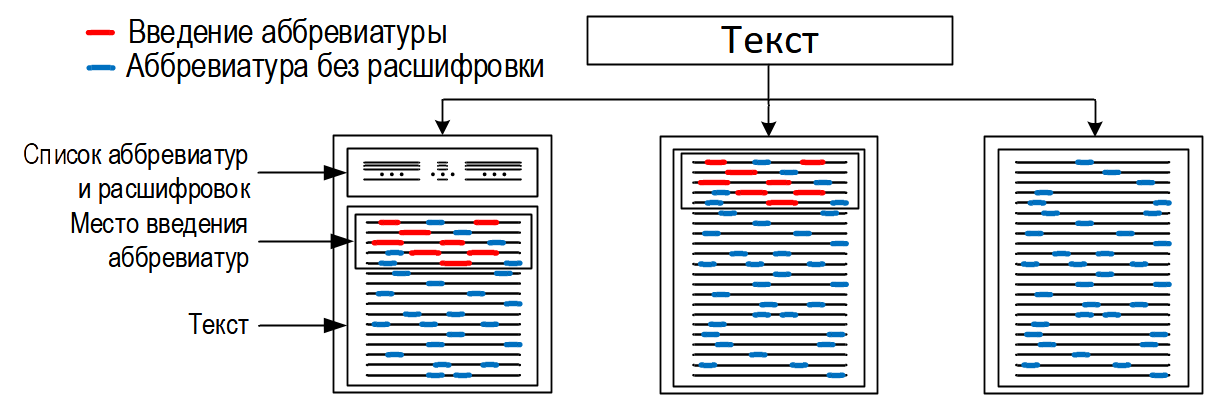
\includegraphics[width=\linewidth]{image.png}
    \label{fig:enter-label}
\end{figure}

\begin{center}
    {\text{{Рисунок 1 – Типы текстов с аббревиатурами (разработано авторами)}} 
\end{center} \\
\hspace{0.6cm}\textbf{2. Состояние предметной области}

\indent В работах [8-10] представляются различные классификации аббревиатур, но не предложено решений по выделению их из текстов. В работе [11] предложено решение для нахождения полного названия журнала по его аббревиатуре. Неизвестная аббревиатура, указанная пользователем, приводилась в формат регулярного выражения, которое предполагало возможный избор слов, начинающийся с указанных букв. Специфическая реализация полученного решения не позволяет использовать его для определения полных форм аббревиатур из других предметных областей.

\indent В работах [2, 13] на основании определения частот встречаемости соседних слов определяется мера их связности, что позволяет предположить вероятные полные формы аббревиатур. Достоинством такого метода является его универсальность, недостатком – высокая трудоёмкость. Материалы данных работ использовались при разработке модели процесса выделения аббревиатур.

\indent В работах [14, 15] предложено исходный текст представлять в виде совокупности тем, которые образуются множеством входящих в них с разной вероятностью слов. Найденная сходимость частей текста используется как представление полной формы аббревиатуры. Данный подход предлагает множество решений с близкими вероятностями, что предусматривает дополнительную работу для пользователя на стадии отбора расшифровки интересующей аббревиатуры.

\indent Существуют программы для ЭВМ, зарегистрированные в Федеральной службе по интеллектуальной собственности

\indent (Роспатент), обладающие возможностью выявления САиР. Так, программа [16] реализует функцию автоматизированного формирования перечня аббревиатур, решает задачу формирования единой базы терминов (аббревиатур) и их определений (расшифровок). Программа [17] предназначена для автоматизированного извлечения терминологических структур из монографии заданной предметной области. С одной из основных функций программы является извлечение терминов, в частности, расшифровка аббревиатур. \\

\textbf{3. Классификация аббревиатур}

\indent Формирование классификации аббревиатур осложнено особенностями их структуры, большой вариативностью, множеством различных способов аббревиации, а также взаимодействием аббревиации с другими способами словообразования. Исследователи [10, 18, 19] сходятся во мнении, что аббревиатуры можно подразделять на инициальные, сложносокращённые и общепринятые. В первом случае аббревиатура составляется из первых букв её расшифровки. Во втором случае в аббревиатуру включены не только первые, но и другие буквы сокращаемых слов [20]. В третьем случае аббревиатуры имеют уникальное представление в тексте и единственную расшифровку. Общепринятые аббревиатуры, как правило, интуитивно понятны и употребляются перед определёнными структурами в тексте.
ция аббревиатур по структурно-информационным признакам (разработано авторами)} 

\indent Для решения задачи автоматизированного ВАиР из текста введём классификацию по структурно-информационным признакам, а также приведём в первом приближении их распространенность, изученную на материале ста случайно отобранных статей с ресурса Cyberleninka.ru. Аббревиатуры разделяются на три класса: инициальные, общепринятые и сложносокращённые. Инициальные и общепринятые аббревиатуры имеют выраженную структуру (прописные буквы, знаки препинания), которой сложносокращённые не обладают (структурный признак). При этом, общепринятые аббревиатуры имеют интуитивно понятный смысл, а инициальные требуют расшифровки в тексте (информационный признак). Сложносокращённые аббревиатуры, не имеющие в составе прописных букв (завхоз, ликбез и т.д.), рассматриваться в данной статье не будут. Инициальные аббревиатуры разделены на пять типов, каждый из которых отличается по структурным признакам (рисунок 2). 
\indent \\
\indent \\
\indent \\
\indent \\
\indent \\
\begin{figure}[h!]
    \centering
    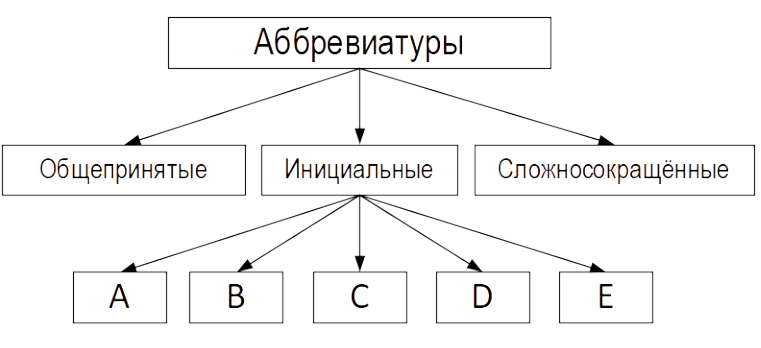
\includegraphics[width=\linewidth]{image2.png}
    \label{fig:enter-label}
\end{figure}

\begin{center}
    {Рисунок 2 – Классификация аббревиатур по структурно-информационным признакам (разработано авторами)} 
\end{center} \\

\indent Для создания программного средства ВАиР необходимо учитывать особенности каждого класса рассматриваемых аббревиатур.
Особенности инициальных и общепринятых аббревиатур:

    1. (Тип А, 53\%) Инициальная аббревиатура, в которой слова полной формы разделены только пробелами и в нее входят только первые буквы слов полной формы. Например: Центр информационной безопасности (ЦИБ), Latent Dirichlet Allocation (LDA).

    2. (Тип В, 5\%) Инициальная аббревиатура, в которой некоторые слова полной формы объединены знаком дефис или символом «косой черты». Например: оптико-тепловизионный комплекс (ОТК), read-only memory (ROM), input/output (I/O).

    3. (Тип C, 22\%) Инициальная аббревиатура с элементами сложносокращённых слов. При этом, аббревиатура может состоять не только из прописных букв, но первая буква полной формы должна соответствовать первой букве аббревиатуры. Количество слов в расшифровке не совпадает с количеством букв в аббревиатуре. Например: гидрометеорологическая станция (ГМС), ammonium bifluoride (АВF), Белорусский автомобильный завод (БелАЗ), временно исполняющий обязанности (ВрИО).

    4. (Тип D, 5\%) Инициальная аббревиатура, отличная от языка документа. Например, протокол передачи файлов (FTP), временный идентификационный номер подвижного абонента (TMSI).

    5. (Тип Е, 2\%) Инициальная аббревиатура, в которой буквы аббревиатуры разделены точками, а первые буквы слов полной формы соответствуют буквам в аббревиатуре. Например: Фамилия Имя Отчество (Ф.И.О.), Петроградская сторона (П.С.).

    6. Общепринятые аббревиатуры (13\%), которые применяются в разных областях: адреса (г., ул., д., пр-т), звания (к-т, д-т), точные науки (см, Гц), время суток (a.m, p.m), элемент текста (P.S.) и т.п. Они не имеют полной формы в тексте и будут расшифровываться по словарю.

\indent Для примеров были использованы аббревиатуры на русском и английском языках, но предполагается, что данная классификация актуальна и для других алфавитных языков.

\vspace{1cm}

\textbf{4. Модель процесса выделения аббревиатур и расшифровок из текста}

\indent Процесс выделения аббревиатур и их расшифровок в общем может состоять из двух этапов.

\indent \textbf{Первый этап} заключается в разделении исходного текста на предложения. Он необходим для более точного определения расшифровок аббревиатур. Разделителем предложений в тексте могут являться восклицательные и вопросительные знаки, многоточия, знаки переноса строки и точки. Однако возникает ряд проблем, связанных с тем, что точки ставятся в тексте не только в конце предложения. Чаще всего точки можно встретить в следующих конструкциях: в датах (25.10.20 г.), в адресах (ул. Ленина, д. 7), в общих аббревиатурах (т.д.), в буквенно-цифровых обозначениях (66.КП.ВРБ.00.00.00 ВО), перед номерами телефонов (тел. 89997773737), в нумерациях (1.1, 1.2, ...), в составе сокращения ФИО (А.А. Иванов) и в инициальных аббревиатурах (R.I.S.K).

\indent \textbf{Второй этап} разбивается на две параллельных части: поиск мест введения аббревиатур и поиск аббревиатур без расшифровок в предложениях.

\indent Поиск мест введения аббревиатур заключается в анализе предложения на предмет наличия аббревиатуры и соответствующей расшифровки. В случае успеха информация о расшифровке и соответствующей аббревиатуре заносится в базу данных. Одна аббревиатура вводится в тексте только один раз.

\indent Введения аббревиатур имеют определенную структуру, которая задается формулой (таблица 1) [3]. Возможны ситуации, когда при введении аббревиатуры в скобках может присутствовать текст, который не относится ни к расшифровке, ни к аббревиатуре.

\begin{table}[h!]
\centering
\caption{Таблица 1 – Типовые формулы введения аббревиатур}
\begin{tabular}{|>{\centering\arraybackslash}p{4cm}|>{\raggedright\arraybackslash}p{8cm}|}
\hline
\textbf{Формула введения} & \textbf{Примеры} \\
\hline
расшифровка (аббревиатура) & Специальное программное обеспечение (СПО), система (С) \\
\hline
аббревиатура (расшифровка) & АС (автоматическая сигнализация), СО (сигнал ожидания) \\
\hline
расшифровка – аббревиатура & Процессор преобразования матриц ППМ, двухпроцессорная система ДС \\
\hline
аббревиатура – расшифровка & ЯМД – язык манипулирования данными, ЯУ – язык управления \\
\hline
(расшифровка – аббревиатура) & (Главная машина – ГМ) \\
\hline
\end{tabular}
\end{table}

\indent Поиск аббревиатур без расшифровок заключается в определении по определенным признакам наличия аббревиатур в предложении.

\indent В процессе поиска могут встречаться аббревиатуры, которые ранее не были введены в тексте. В связи с
вязи с этим появляется необходимость поиска информации об их расшифровках по другим источникам. Для корректного сопоставления аббревиатуры и расшифровки из разных текстов, необходимо учитывать контекст аббревиатур (рисунок 3).

\begin{figure}[h!]
    \centering
    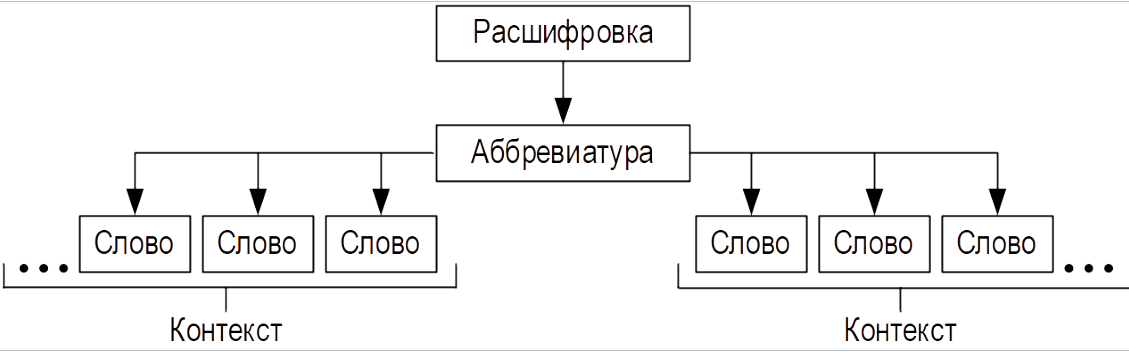
\includegraphics[width=1\linewidth]{image3.png}
    \label{fig:enter-label}
\end{figure}
\vspace{3cm}
\begin{center}
    {(Рисунок 3 – Соответствие расшифровки, аббревиатуры и контекста (разработано авторами)} 
\end{center} \\
\indent Так как одна аббревиатура вводится в тексте, как правило, только один раз, то далее по тексту будут встречаться только аббревиатуры без расшифровок, при этом каждая выделенная аббревиатура будет однозначно соответствовать введенной ранее. Далее от предложения к предложению необходимо учитывать контекст аббревиатуры и их контекст в базу данных, после чего производить сопоставление с информацией, полученной при поиске мест введения предложения.

\begin{figure}[h!]
    \centering
    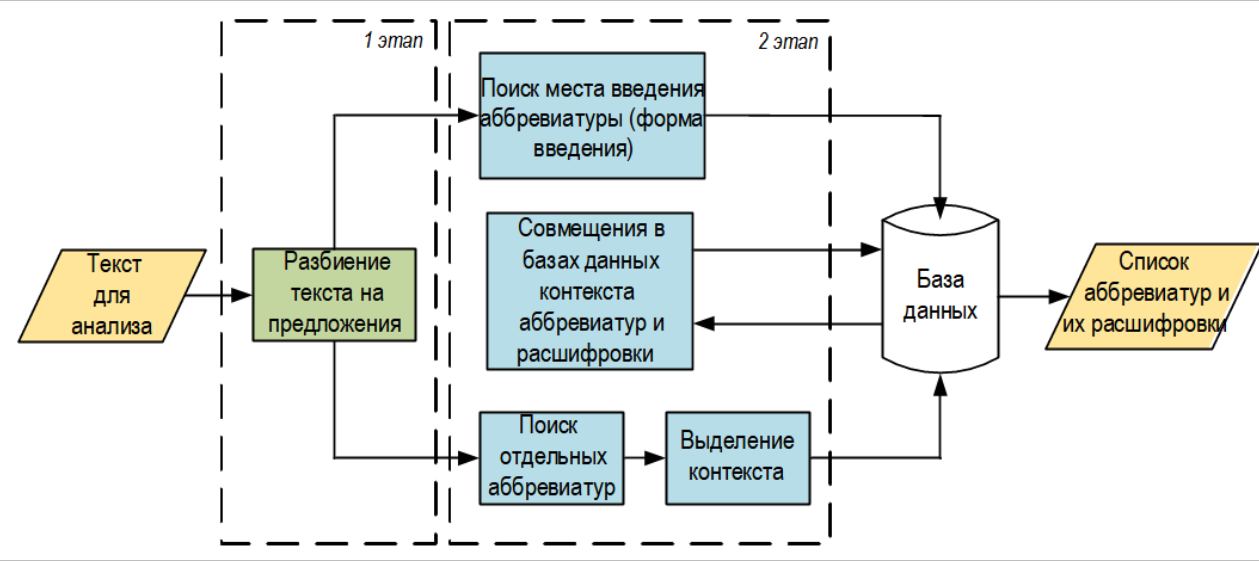
\includegraphics[width=1\linewidth]{image4.png}
    \label{fig:enter-label}
\end{figure}
\begin{center}
    {(Рисунок 4 – Принципиальная схема выделения аббревиатур и расшифровок в тексте (разработано авторами))} 
\end{center} \\
\indent \\
\indent \\
\indent \\
\section{\large Заключение}

В статье рассматривается обобщенное гиперболическое уравнение запаздывающего типа с некарлемановскими сдвигами вида:

\begin{equation}
    u_{xx}(x,y) - u_{yy}(x,y) = H(x - \tau)[U_x(x - \tau, y)] + U(x - \tau, y). \tag{1}
\end{equation}

где в области

\begin{equation}
    D = \{(x, y) : x > 0, y < \alpha\}, \quad \alpha = \bigcup_{k} D_k
\end{equation}

\begin{equation}
    D_k = \left\{(x, y) : k\tau - \gamma \leq x \leq (k + 1)\tau + \gamma, -\frac{\gamma}{2} < y < \frac{\gamma}{2} \right\}, \quad (k = 0, 1, 2, \dots)
\end{equation}

\textbf{Задача K.} Найти в области $D$ решение уравнения из класса $C(\overline{D}) \cap C^2(D)$, удовлетворяющее условиям

\begin{equation}
    U(x, y)|_{y=0} = \omega(x), \quad x \geq 0, \tag{2}
\end{equation}

\begin{equation}
    U_y(x, y)|_{y=0} = \nu(x), \quad x > 0, \tag{3}
\end{equation}

где $\omega(x), \nu(x)$ – заданные непрерывно достаточно гладкие функции, причем $\omega(x) > \omega(t + \tau) \geq 0$.

\begin{center}
    {\textbf{{Список литературы}} 
\end{center}
\noindent    1. Максименко, О.И. Новые тенденции аббревиации (на материале русского, английского и немецкого языков) // Вестник Российского университета дружбы народов. Серия: Теория языка. Семиотика. – (семантика). – 2017. – Т. 8. – № 1. – С. 174-181.
    
\noindent     2. Грихуцина, Т.А. Лингвистические проблемы автоматизации редакционно-издательских процессов / Т.А. Грихуцина, Н.П. Дерчук, Л.И. Комарова и др.; отв. ред. В.И. Перебейнос, М.Д. Феллер // колл. монография; Академия наук УССР, Институт языковедения им. А.А. Потебни. – Киев: Наукова думка, 1986. – 229 с.
    
\noindent     3. Гращенко, Д.А. Информационные основы польско-русского межъязыкового преобразования текстов / Д.А. Гращенко, Н.Н. Пивоваров // Новые информационные технологии и технологии автоматизированных систем. – 2016. – № 19. – С. 101-106.
    
\noindent     4. Мизернов, И.Ю. Анализ методов оценки сложности текста / И.Ю. Мизернов, Д.А. Гращенко // Новые информационные технологии в автоматизированных системах. – 2015. – № 18. – С. 572-581.
    
\noindent     5. Ванюшкин, А.С. Методы и алгоритмы извлечения ключевых слов / А.С. Ванюшкин, Д.А. Гращенко // Новые информационные технологии в автоматизированных системах. – 2016. – № 19. – С. 85-93.
    
\noindent     6. Науменко, Д.А. Информационные основы автоматизации рерайтинга / Д.А. Науменко, Л.А. Гращенко, Г.В. Романишин // Новые информационные технологии в автоматизированных системах. – 2019. – № 22. – С. 187-191.
    
\noindent     7. Гращенко, Л.А. Опыт автоматизированного анализа повторов в научных текстах / Л.А. Гращенко, Г.В. Романишин // Новые информационные технологии в автоматизированных системах. – 2015. – № 18. – С. 582-590.

\noindent     8. Суперанская, А.В. Общая терминология: Вопросы теории. Аббревиация в терминологии / А.В. Суперанская, Н.В. Подольская, Н.В. Васильева. – Изд. 6-е. – М.: Книжный дом «ЛИБРОКОМ», 2012. – 248 с.

\noindent     9. Нургалеева, Т.Г. Аббревиация как средство экспрессивного словообразования: автореф. дис. канд. филол. наук, спец. 10.02.04 «Германские языки» / Т.Г. Нургалеева. – М.: Наука, 2016. – 240 с.

\noindent     10.Земская, Е.А. Современный русский язык. Словообразование: учеб. Пособие. 3-е изд., испр. и доб. – М.: Наука, 2011.

\noindent     11. Jenkins K. Deciphering Journal Abbreviations with JAbbr // Code4Lib Journal. – 2009. – № 7. [Электронный ресурс] URL:https://journal.code4lib.org /articles/1758 (Дата обращения: 09.11.2021).

\noindent     12. Mikolov T. Efficient Estimation of Word Representations in Vector Space / T. Mikolov, K. Chen, G. Corrado, J. Dean // arXiv.org. – 2013. [Электронный ресурс]

\noindent     URL:http://arxiv.org/pdf/1301.3781v3.pdf (Дата обращения: 10.11.2021).

\noindent     13. Mikolov T. Distributed Representations of Words and Phrases and their Compositionality / T. Mikolov, I. Sutskever, K. Chen, G. Corrado, J. Dean // Advances in Neural Information Processing Systems. – 2013. – P. 3111-3119.

\noindent     14. Bleil, D.M. Latent Dirichlet Allocation / D.M. Bleil, A.Y. Ng, M.I. Jordan // Journal of Machine Learning Research. – 2303. – № 3. – P. 993-1022.

\noindent     15. Heinrich G. Parameter estimation for text analysis. — 2004. [Электронный ресурс] 

\noindent     URL:http://citeseerx.ist.psu.edu/viewdoc/summary?doi=10.1.1.216.695

\noindent     (Дата обращения 10.11.2021)

\noindent     16. Автоматизированное формирование перечня аббревиатур (сокращений) / А.А. Чумичкин, М.В. Руты, Г.И. Трифонов // Свидетельство о регистрации программы для ЭВМ RU 2018663069, 19.10.2018. Заявка № 2018660897 от 04.10.2018.

\noindent     17. Программа для извлечения и анализа терминологических структур смежных предметных областей / Д.А. Губанов // Свидетельство о регистрации программы для ЭВМ RU 2019665358, 22.11.2019. Заявка № 2018664640 от 18.11.2019.

\noindent     18. Алексеев, Д.И. Сокращенные слова в русском языке. – Саратов: Изд-во Саратовского ун-та, 1979. – 328 с.

\noindent     19. Виноградова, В.В. Русская грамматика: научные труды. В 2 т. Т. 1 – М.: Российская академия наук, 2005. – 784 с.

\noindent     20. Ахманова, О.С. Словарь лингвистических терминов. — М.: Едиториал УРСС, 2004. – 576 с.
    
\end{document} % Required for inserting images